\documentclass[10pt,a4paper]{article}
%\documentclass[10pt,a4paper]{beamer}
\usepackage[utf8]{inputenc}
\usepackage{amsmath}
\usepackage{amsfonts}
\usepackage{amssymb}
\usepackage{graphicx}
\usepackage[left=2cm,right=2cm,top=2cm,bottom=2cm]{geometry}
\usepackage{kpfonts}
\usepackage[justification=centering]{caption} %to adjus caption center aligned
\usepackage{hhline} %to add double horizontal line in tabular
\usepackage[numbers]{natbib}
%other options include: round, curly, angle, or default options
\usepackage{media9} %package for include movies
\author{Zhixuan Cao, Abani Patra}
\title{Data Management and Domain Adjusting Strategies for Implementing Parallel SPH Method in JPUE Simulation}

\begin{document}

\maketitle
%\tableofcontents
\section{Abstract}
This paper presents a parallel implementation of smoothed particle hydrodynamics (SPH) method using the message passing interface (MPI) standard to simulate a turbulent jet or plume which is ejected from a nozzle into a uniform environment(JPUE). Background grid is used to reduce neighbors searching cost and decompose (redecompose) the domain. Hilbert Space Filing Curve(SFC) based index is adopted to assign an unique identifier to each background grid. As simulation of JUPE requires adding of new particles during simulation, time-dependent SFC indexes are assigned to particles to guarantee uniqueness of identifier.  
%to distinguish particles added at the same position but different simulation time step. 
Both particle and background grid are stored in hashtables. Additional link list attached to the hashtable is used to handle hash confliction. A dynamic domain decomposition strategy is implemented to ensure good load balance. Furtherly, computational domain is adjusted during simulation to reduce computational cost. 
Numerical tests show that our code has good strong scalability.
These strategies can be further applied to many other implementations of meshfree methods, Especially those implemetations that require flexible accessing, adding and deleting of particles.
\section{Introduction}
SPH is a meshless scheme, initially developed for astrophysical applications by Lucy\citep{lucy1977numerical} and Gingold and Monaghan\citep{gingold1977smoothed}. 
Subsequently it was extended to large strain solid mechanics and computational fluid mechanics. 
A lot of research has been done in parallellization of SPH. 
Goozee\citep{goozee2003distributed} implemented a simple SPH code using MPI, OpenMP and BSP. 
Chen Wenbo\citep{wenbo2014performance} presented a parallel SPH implementation on multi-core CPUs. 
Jose M. David W. Holmes\citep{holmes2011framework} presented a simulation framework that enables distributed numerical computing in multi-core shared-memory environments. 
Domínguez\citep{dominguez2011optimization} present optimizations for both CPU and GPU parallelization of a SPH method. 
Angela Ferrari\citep{ferrari2009new} parallelized a 3D SPH code using the message passing interface (MPI) standard, together with a dynamic load balancing strategy to improve the computational efficiency of the scheme. 
D. Kumar and Abani\citep{kumar2013parallel} implemented CPU parallel Godunov SPH in simulation of granular flows.
A.J.C. Crespo\citep{crespo2015dualsphysics} used the parallel power computing of GPUs to accelerate DualSPHysics by up to two orders of magnitude compared to the performance of the serial version.\\
However, most implementation of parallel SPH method is limitted to bechmark problems like dam break, or relative simple scenarios like breaking-waves, floodings ect. Rare work has been done in simulation of more complicated problems, such as eruption of volcano plume which is essentially a mutilple phases, turbulent, ejection flow process accompanied with microphysics phenomena like phase change of water, aggregation, reaction ect. Prediction of such more complicated phenomena with acceptable accuracy at given time window can not been acomplished without parallel computing. Imposing of boundary conditions (such as realistic wind feild, eruption boundary condition and no-slip wall boundary condition) requires dynamiclly adding and removing of particles during simulation. This requies efficient and more flexible data management scheme. In this paper, we implement SPH to simulate a simplified version of this complicated volcanic plume: JPUE. and develop data management methodologies for it.\\
Among existing CPU parallel SPH schemes, most of them focus on neighbor searching algorithm and dynamic load balancing.  (eg.\citep{ferrari2009new, crespo2015dualsphysics}). Less attention has been paid to developing of more flexible data structures for more complicated problem. 
Fortunately, efficient and flexible data management strategies for high performance computing have been successfully implemented in meshbased methods(eg. \citep{laszloffy2000simple} for adaptive hp FEM, and \citep{pitman2003computing, patra2005parallel} for FVM). Motivated by techniques developed for mesh based methods, we present a complete framwork for parallelizing SPH program with MPI standard model allowing more flexible and efficient data access in this paper.\\
Any implementation of SPH code requires efficient searching and updating of neighbors during simulation. We adopted background grid which was proposed by Monaghan and Lattanzio\citep{monaghan1985refined} and implemented widespreadly in parallel SPH. The background grid is also used for domain decomposition in SPH. We refer to the elements of background grid, namely a squares for two dimension and cubics for three dimension, as buckets. As for the storage of physical quantities associated to each particle, different strategies was adopted in existing implementation of SPH. 
In both SPHysics\citep{dominguez2011optimization} and DualSPHysics\citep{crespo2015dualsphysics}, The physical quantities of each particle (position, velocity, density…) are stored in arrays, and the particles (and the arrays with particle data) are reordered following the order of the cells. This has two advantage: 1)access pattern is more regular and more efficient, 2) It is ease to identify the particles that belongs to a cell by using a range since the first particle of each cell is known. But adding, deleting and especially accessing of particles are cumbersome. Angela Ferrari\citep{ferrari2009new} adopted linked lists using pointers so that particles can be deleted or added during the simulation. Storage problems caused by fix-size arrays are thereby also eliminated. We define C++ classes which contains all data of particle and bucket. As for the storage of data, we adopt an hashtable to store pointers to particles and buckets, which gives us not only flexibility of deleting and adding element, but also quicker access compared with linked list. Instead of using the "nature manner" to number particles, we adopt SFC based index to give each particle and background bucket an unique identifier. The SFC based numberring strategy is further extended to include time step information so that particles added at the same position but different time will have a different identifier. As for domain decomposion, even though more complicated graph-based partition tools\citep{biswas1999experiments} might get higher quality decomposition, they requires much more effort in programming. So we adopt an easy-programming scheme based on SFC \citep{patra1999efficient}.\\
To the best of the author's knowledge, no implementation of SPH has the feature of adjusting computational domain based on simulation. For JPUE simulation, such feature will greatly reduce computational cost by avoiding computing of uninfluenced fluid. This feature is accomplished by adding a scan function to monitor the most outside layer of the domain and turn ghost particles to real particles at proper time. 
%The computational cost of this additional scan function is low.
\\
The data structure, particle and bucket indexing strategies, domain decomposition and adjusting strategies, and dynamic load balancing method in this paper can be easily adopted by other implementations of any meshfree methods(include SPH). The flexibility of data accessing enables implementing of meshless methods for solving of more complicated problems.\\
%In the following sections, the physics and SPH implementation of inject flow problem is given, then 
\section{Data structure and load balance}

\begin{figure}[h]
\caption{Basic Work flow for SPH}
\centering
\label{fig:Work_flow}
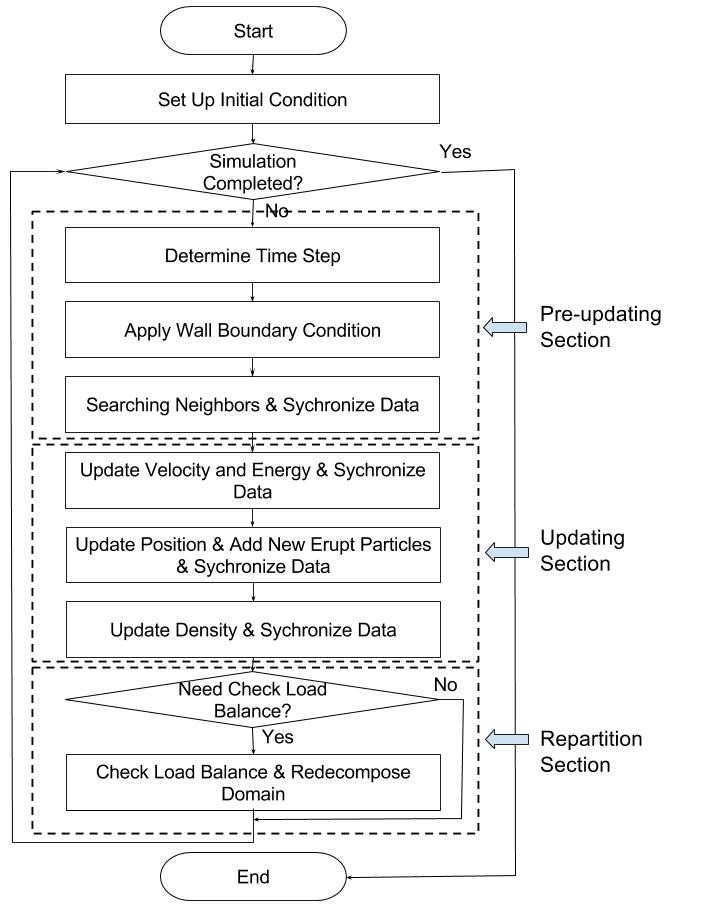
\includegraphics[width=0.5\textwidth]{Work_flow}
\end{figure}

SPH is a meshfree, Lagrangian method. The domain is discretized by particles and the position of particle is updated at every time step. The physical laws (such as conservation laws of continuum fluid dynamics) written in the form of partial differential equations need to be transformed into the Lagrangian formalism. Using a kernel function that provides the weighted estimate of the field variables at a discrete point (particle), the integral equations are evaluated as sums over neighbor particles. Only particles located within support of kernel function will interact. Thus, physical proterties (position, density, velocity, internal energy, pressure) are updated based on its neighbors. So a neighbor searching need to be carried out before updating of physical proterties. We use buckets which overlap the whole domain and keep fixed in time during the entire simulation, to reduce searching cost. Domain decomposition will be based on SFC going through centroid of buckets. A basic works flow of our SPH code is shown in figure \ref{fig:Work_flow}.\\

Particles need to be added and(or) removed during simulation of JPUE problem. Wall boundary conditions in SPH can be imposed either by adding a force term or using ghost particles. We adopt the latter one in our simulation. As our computational domain will be adjusted during simulation, wall ghost particles need to be added or deleted during simulation. New particles also need to be added for the eruption boundary condition. 
We will describe in this section these strategies which allows flexible deleting and adding.
\subsection{SFC based indexing}
Our data structure start from assigning each particle and bucket an identifier, we refer to it as key, which should be unique throughout simulation. The key for bucket is determined by centroid coordinates of the bucket while the key for particle is determined by adding coordinates and adding time step. The map from coordinates to key is based on SFC.\\
The SFC \citep{sagan2012space} maps n-dimentional space to a one dimentional sequence. The standard procedure for obtainning SFC is: 
\begin{itemize}
\item Scale coordinates of particle or bucket into $[0,1]^n $ based on maximum and minimum coordinates of the computational domain: $\textbf{X}^\prime \rightarrow \textbf{X}$
\item Computed $k_r = h_n(\textbf{X})$. Where $h_n$ is the map $h_n: [0,1]^n \rightarrow [0,1]$. 
\item Convert $k_r$ to integer $k$ by multiplying $k_r$ with a very large number and removing decimal part.
\item All keys are sorted to form a sequence which is SFC. SFC represents a curve passing through all particles (or centroid of buckets).

\end{itemize}
{
\begin{figure}[h]
\caption{Spcace filling curve orderings of buckets and particles in the buckets}
\centering
\label{fig:SFC_particles_buckets}
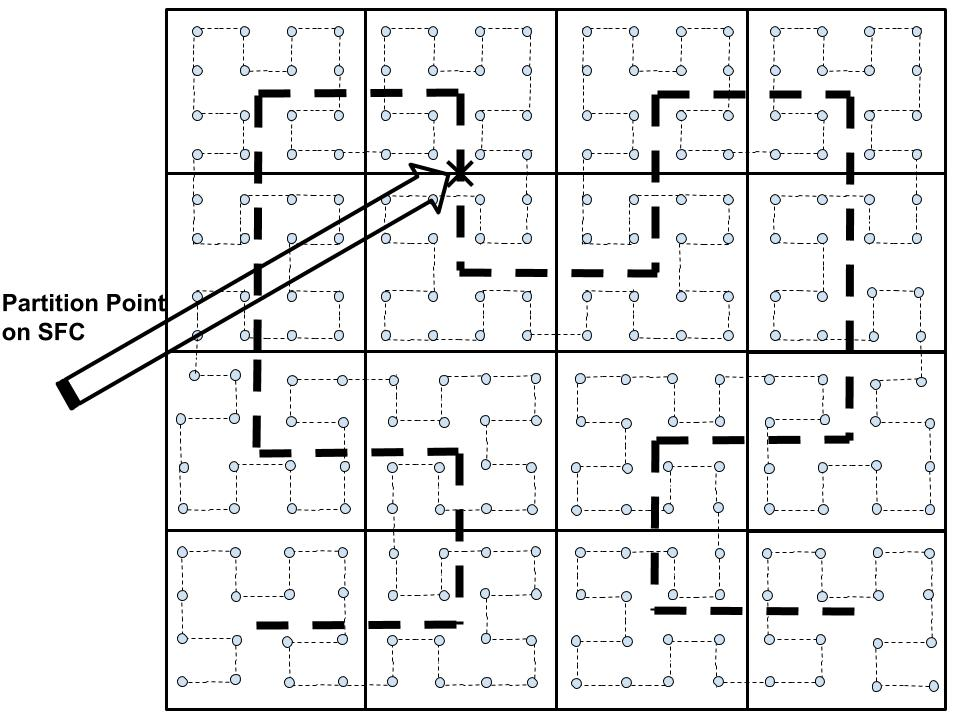
\includegraphics[width=0.6\textwidth]{SFC_particles_buckets}
\end{figure}

\begin{figure}[h]
\caption{Decomposition of domain based on SFC}
\centering
\label{fig:SFC_particles_buckets_partition}
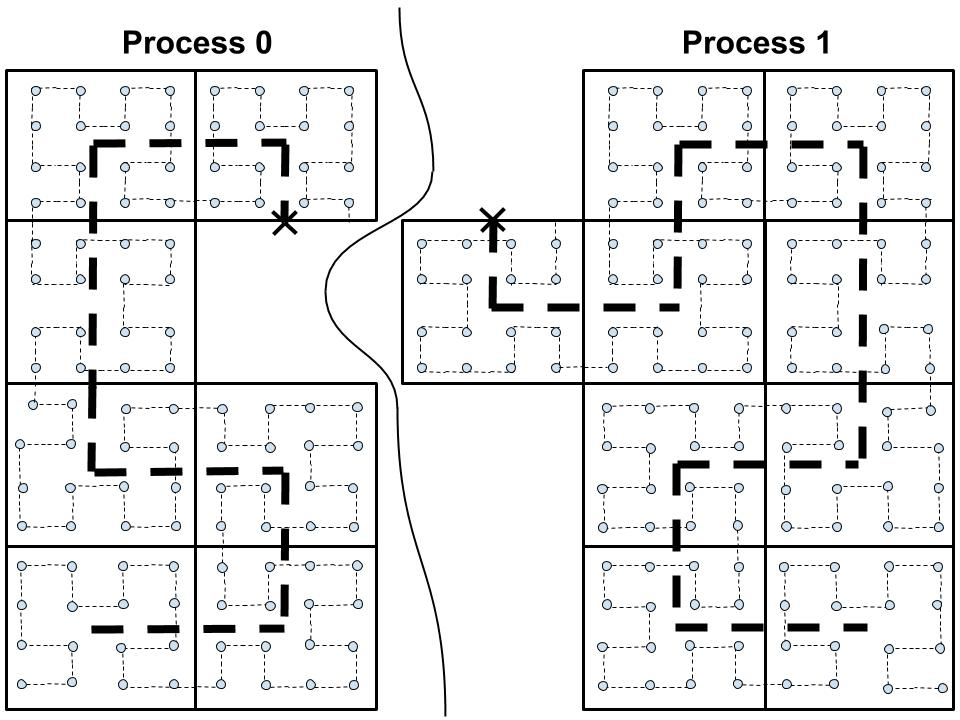
\includegraphics[width=0.6\textwidth]{SFC_particles_buckets_partition}
\end{figure}
}

Scheme for constructing the map $h_n$ can be found in \citep{patra1995problem}. These keys denote a simple addressing/ordering scheme for the data and computations, i.e., a simple global index space for all the objects.\\
SFC-based indexing scheme can guarantee uniqueness of particle identifier only in simple scenarios when particles are added once while setting up initial condition. In some situations, new particles need to be added while simulation. For example, new particles need to be added at the bottom of the eject vent to simulate JPUE. To distinguish particles added at the "same place" (the small area, all points whithin which will be mapped to the same $k$.) from different time steps, we extend the SFC-based key to SFC based time-dependent key by including date of birth of particles into the key. The SFC based time-dependent key can be written as: $[k,t]$, where $t$ is the time step. The map $h_n$  will become: 
$h_n: [0,1]^n \times \textbf{T} \rightarrow [0,1] \times \textbf{N}$
where $\textbf{T} \subset [0,\infty)$ is the time step dimension, $\textbf{N}=\lbrace 0, 1, 2, 3...\rbrace$.
To guarantee locality, sorting of particle keys is majorly based on $k$, that is to say, particle with smaller $k$ always comes before particles with larger $k$. For these particles has the same $k$, ordering of them will depend on $t$. Figure \ref{fig:SFC_particles_buckets} shows SFC ordering of buckets and particles in buckets. 
Several features of such indexing scheme are suitable for SPH:
\begin{itemize}
\item Guarantee uniqueness of identifier.
\item Key of each object is generated purely based on its own coordinates. While add new objects on different processes, key of each object can be generated fast and independently .
\item Objects that locate closely in the Euclidian space will also be close to each other in the one dimensional key space in the mean sense. Since SPH particles only interact with its neighbors, geometric locality can be exploited for efficient storage and retrieval of bucket and particle data.
\item This type of key effectivelly generate a global address space. Globality of key and conservation of locality make it easy to partition the sorted key squence and obtain the decompositiion of the problem.
\end{itemize}
What need to point out is that motion of particles might mess up locality that established based on initial coordinates of particles. As particles are moving regularly, the locality of most of particles should still be conserved during simulation.
%If we can design a re-numberring method which is computationally cheap, we can restore the locality.
\subsection{Data structure}
\subsubsection{Particle and bucket}
The most basic data structure of SPH are particle, for problem discription, and bucket, for neighbor searching and domain decomposition. Both are defined as classes in C++. Infomation that contained in particle class can be categorized into six categorise: ID(the key), affiliate(process that the particle belong to), primitive variables (variables show up as unknows in governing equations, like coordinates, density, velocity, energy), secondary variables (properties that can be computed from primitive variables, they are stored to avoid repeatedly computing, eg. pressure, temperature ect.), flags (indicators, such as indicator for ghost particle and real particles, indicator for particles of different phases ect.) and neighbor infomation (it is vector of particle keys in our application). Similarly,  Infomation that contained in bucket class can also be categorized into different categorise: ID(the key), affiliate(process that the bucket belong to), domain information (maximum and mimnum coordinates, boundary infomation), flags (indicators, such as indicator for guest and non-guest, indicator for active and inactive), neighbor infomation (27 neighbor buckets including itself for three dimension and 9 for two dimension). Objects defined based on these two classes are then accesse through hash tables.
\subsubsection{Hash table and hash confliction}
As discussed at the beginning of this section, implementation of SPH in more realistic scenarios requires dynamic memory management and flexible data access. One of the fundemental data structures that satisfy such requirement is hash table. Another option is B-tree. We adopt hash table. An implementation of B-tree under a similar situation for mesh based methods can be found in other papers(eg.\citep{patra2003data}).\\
Hash table, which is divided into slots, are array based data structure. Based on the key, the address-calculator(hashing) function determines in which slot the data should be stored. The hashing function maps from key to the slot index:
\begin{equation}
slot\,index = hash(key)
\end{equation}
The hash table has O(1) data accessing, adding and delete properties when there is no confliction. How many conflictions will happen depends on both distribution of keys in the keys space and size of the hash table. As the distribution of keys is determined by particles' initial location (or centroids of buckets), the hash table size is under our control. We can use very large hash table to minimize hash confliction on the expense of sparse data distribution which will lead to low prefetch and low memory efficiency. Or oppositely, we can use smaller hash table size to obtain high memory efficiency on the expense of having many hash confliction. Abani\citep{patra2003data} did numerical experiments to make trade-off to determine hash table size.\\
 %We should also do some experiment to optimize our hash table size.
One way to handle hash confliction is using an additional sorted vector attached to the hash table. When several keys hash to the same slot, a vector will be created. The vector is sorted based on keys so that a binary search can be used to find the correct position for adding, deleting or retrievaling . Another option to handle hash confliction is using an additional link list which is more flexible in memory allocation. The average time complexity of binary search is O(log n) while that for linear search based on link list is O(n). However, accessing efficiency of link list is much lower than array based data structure, especially when the link list becomes longger. Choosing of proper way to handle hash confliction greatly depends on the problem itself. For the test problem in this paper, successively adding of particles at the bottom of the eject vent will lead to hash confliction of many particles, which implies a long link list. But considering the very long conflictions only occur on several slots among millions (see figure \ref{fig:Particle_adding_with_link}), we still choose the link list to handle the hash confliction. This decision was made based on numerical experiments.
\subsubsection{Hash function}
\begin{figure}[h]
\caption{Ununiform distribution of particles in the $[0,1]^n \times \textbf{T}$ space due to adding of new particles at a small portition of the domain, these new particles will be stored in external link list}
\centering
\label{fig:Particle_adding_with_link}
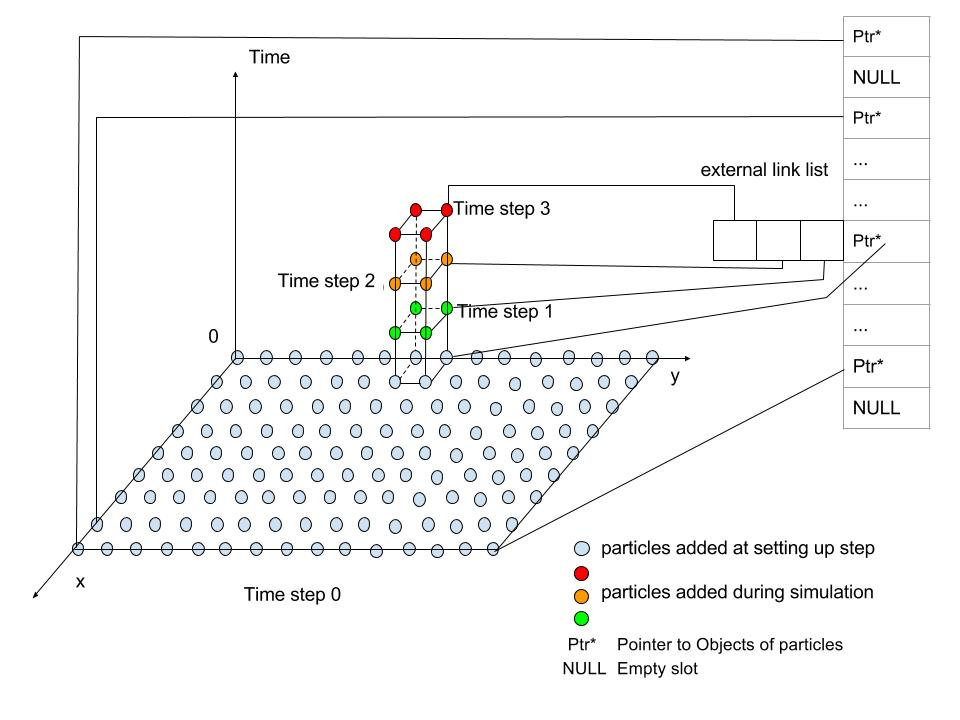
\includegraphics[width=0.6\textwidth]{Particle_adding_with_link}
\end{figure} 
For time-independent keys, the hash function can be a simple function like:
\begin{equation}
\label{eq:hash_function}
slot\,index = \frac{Key - Min\,Key}{Max\,Key - Min\,Key} \times Hash\,Table\,Size 
\end{equation}
One natural way to hash SFC based time-dependent key $[k,t]$ is to convert the two elements in the key into one number taking $k$ as higher digit and $t$ as lower digit of the large number. However, for JPUE simulation, even though ghost particles for wall boundary condition and pressure boundary condition also need to be added during simulation, places for adding of these two types of ghost particles are previsouly empty area. Only ghost particles for eruption boundary condition will be successsively added at the same place: bottom of the vent. That is to say, particles are distributed ununiformly in the $[0,1]^n \times \textbf{T}$ space as show in figure \ref{fig:Particle_adding_with_link}. To avoid ununiform, very sparse hash table and conserve locality of SFC, we only plug the first number $k$ of the key $[k,t]$ into the hashing function, equation (\ref{eq:hash_function}). 

\subsection{Load balance strategy}
\subsubsection{Weighted work load}
Particles in the test problem can be categorized into real particle, wall ghost particle, pressure ghost particle, eruption ghost particle. Ghost particles are for imposing of corresponding boundary conditions (see figure \ref{fig:Involved_initial} and \ref{fig:Involved_domain_adjusting}). As different type of particles involves different amount of computation,shown by table \ref{tab:Computational_cost_particles} and table \ref{tab:Computational_cost_steps}, we assign different work load weight for different type of particles based on profilling data. Work load of each bucket is then determined by summing up work load weight of all particles within the bucket. The SFC sequence passing through centroids of all buckets now become a weighted sequence. Domain decomposition will conducted based the weighted SFC.
\begin{table}[h!]
  \centering
  \caption{Computational cost for different steps per particle}
  \label{tab:Computational_cost_steps}
  \begin{tabular}{|c|r|r|}
    \hline
    Step & Cost ($\mu s$) & Abbreviation\\
    \hhline{|=|=|=|}
    neighbor search & 0.45 & NS\\
    \hline
    update momentum and energy & 0.62 & UPME\\
    \hline
    update density & 0.37 & UPD\\
    \hline
    update position & 0.02 & UPP\\
    \hline
    velocity filtering& 0.38 & VF\\
    \hline
    apply wall bc & 1.2 & WBC\\
    \hline
  \end{tabular}
\end{table}

\begin{table}[h!]
  \centering
  \caption{Computational work load for each type of particle}
  \label{tab:Computational_cost_particles}
  \begin{tabular}{|c|r|r|r|r|r|r|r|}
    \hline
    Particle type & NS & UPME & UPD & UPP &VF &WBC &Total\\
    \hhline{|=|=|=|=|=|=|=|=|}
    Real & Yes & Yes & Yes & Yes & Yes & No & 1.8\\
    \hline
    wall ghost & No & No & No & No & No & Yes &1.2\\
    \hline
    eruption ghost & No & No & No & Yes & No & No & 0.02\\
    \hline
    pressure ghost & No & No & No & No & No & No & 0.\\
    \hline
  \end{tabular}
\end{table}
\subsubsection{Domain decomposition and dynamic load balancing}
Domain decomposition will be conducted based the weighted SFC of buckets. Figure \ref{fig:SFC_particles_buckets} and figure \ref{fig:SFC_particles_buckets_partition} show how domain will be decomposed based on partition of SFC of buckets. The particles are automatically split into two groups along with buckets that contain them. In our current implementation, the domain is partitioned only in $x-y$ plane. A two dimensional footprint of the three dimensional domain(as well as buckets) is generated by projecting. 
%SFC for the two dimensional footprint is partitioned for domain decomposition. 
The work load of each object on the SFC of footprint buckets in $x-y$ plane will be the summation of work loads of all buckets above the footprint. 
Movement of particles, adding of new particles, adjusting of domain will lead to load imbalance between processes. Computational load is monitored at given interval (The interval is optimized based on numerical experiments). Repartitioning is carried out if load imbalance is larger than a given tolenrance. Figure \ref{fig:t0_domain_decomposition} and \ref{fig:t10_domain_decomposition} show the initial decomposition and domain decomposion at 10 seconds. 
%We adopt the same SFC based partition strategy as described by Patra \ref{patra1999efficient}. 
\begin{figure}[h]
\caption{An example of sub-dividing domain into 4 partitions using SFC Partitioning: initial domain decomposition}
\centering
\label{fig:t0_domain_decomposition}
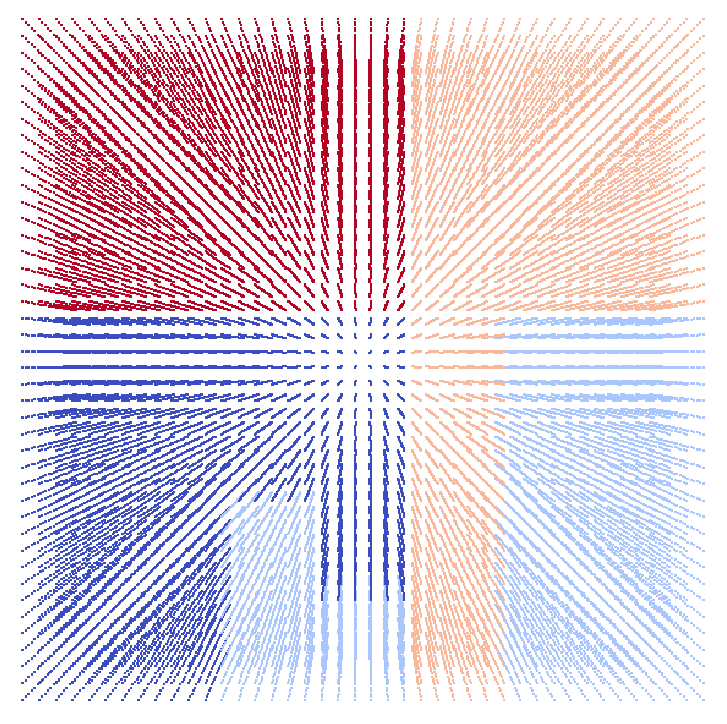
\includegraphics[width=0.5\textwidth]{t0_domain_decomposition}
\end{figure}

\begin{figure}[h]
\caption{An example of sub-dividing domain into 4 partitions using SFC Partitioning: decomposition at t=10s}
\centering
\label{fig:t10_domain_decomposition}
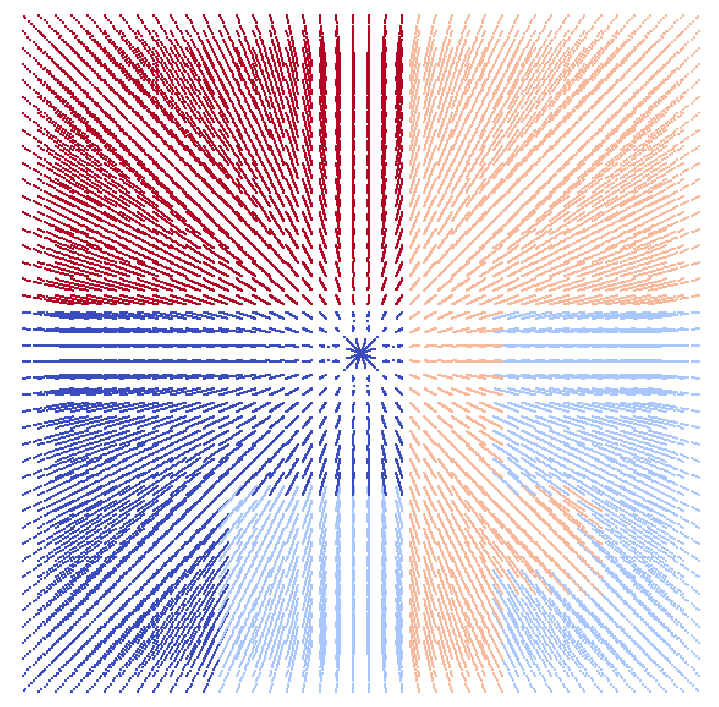
\includegraphics[width=0.5\textwidth]{t10_domain_decomposition}
\end{figure}
As some of the neighbor particles reside in other
partitions. A set of “guest” particles and buckets are used to synchronize data across partitions. To minimize communications, data is synchronized only where needed, using non-blocking MPI communications. 
\section{Adjusting of domain during simulation}
%SPH particles can be viewed as discretization points\citep{diltsg1999moving}. 
As a Lagrangian method, SPH is able to automatically adjust computational domain(eg, dam break simulation) as the postition of the dicretization points are updated at every time step. However, for JPUE simulation, where some fluid ejects into stationary fluid and get mixed due to turbulence, the domain-adjusting feature of SPH will gone. Because the whole domain, which occupied by stationary fluid before eject fluids reaching there, has to be discretized at the very beginning of simulation. A lot of CPU time will be spent on computing of "stationary" particles. It is pure wasting of computational resources. If we can avoid simulating of stationary particls by adjusting the computational domain, the computational cost will be reduced greatly. To the best of the author's knowledge, no implementation of SPH has the feature of adjusting computational domain based on simulation. We proposed a simple strategy to add such feature in our code with low computational cost. We add a scan function to monitor the most outside layer of the domain. When the ejected fluid reaches the boundary of the current domain,  ghost particles (for pressure boundary condition) will be turn to real particles and then add new ghost particles. The original work flow (see figure \ref{fig:Work_flow}) is modified to enable such feature. (see figure \ref{fig:Work_flow_adjust})

\begin{figure}[h]
\caption{Work flow that enables domain adjusting feature}
\centering
\label{fig:Work_flow_adjust}
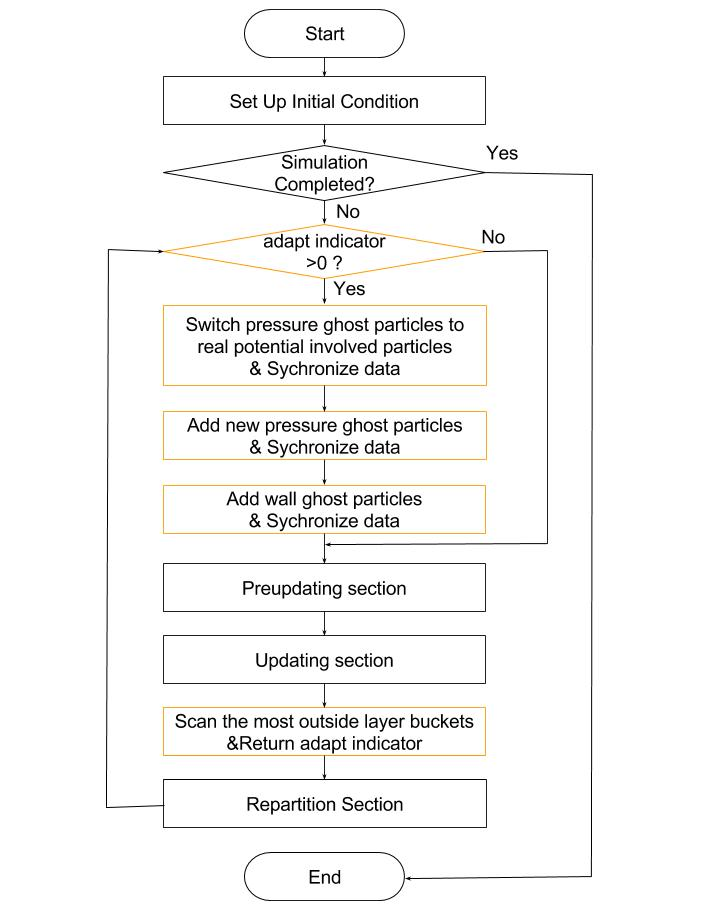
\includegraphics[width=0.5\textwidth]{Work_flow_adjust}
\end{figure}
The start point of adding adjusting feature is adding a flag, which we refer to as involved-flag, into particle class. Particles are categorized into three groups based on the value of the flag: involved (involved-flag=2), potential involved (involved-flag=1), and not involved(involved-flag=0). The involved particles are particles that have already been involved in eject mixing. The potential involved particles are particles that have not been involved in eject mixing but adjecent to involved particles. So they will be involved in the mixing process in the near future. These not involved particles are particles that far away from the eject source and is still at the initial state. For these not involved particles, it is not necessary to update its state variables. As a consequence, searching for neighbors and data communitation for these particles are also unnecessary. That is to say, only potential involved and involved particles need to be simulated.
As simulation goes, the ejected fluid will reach larger area and more and more particles will be influenced. The criteria to determine whether a particle is involved or not is: whether the mass fraction of that particle is larger than a given threshold (10e-5 in out simulation). Other state variable, such velocity, can also serve as alternative "swich criteria".\\

{
\begin{figure}[h]
\caption{Imposing of all kinds of boundary condition, and using of flag Involved}
\centering
\label{fig:Involved_initial}
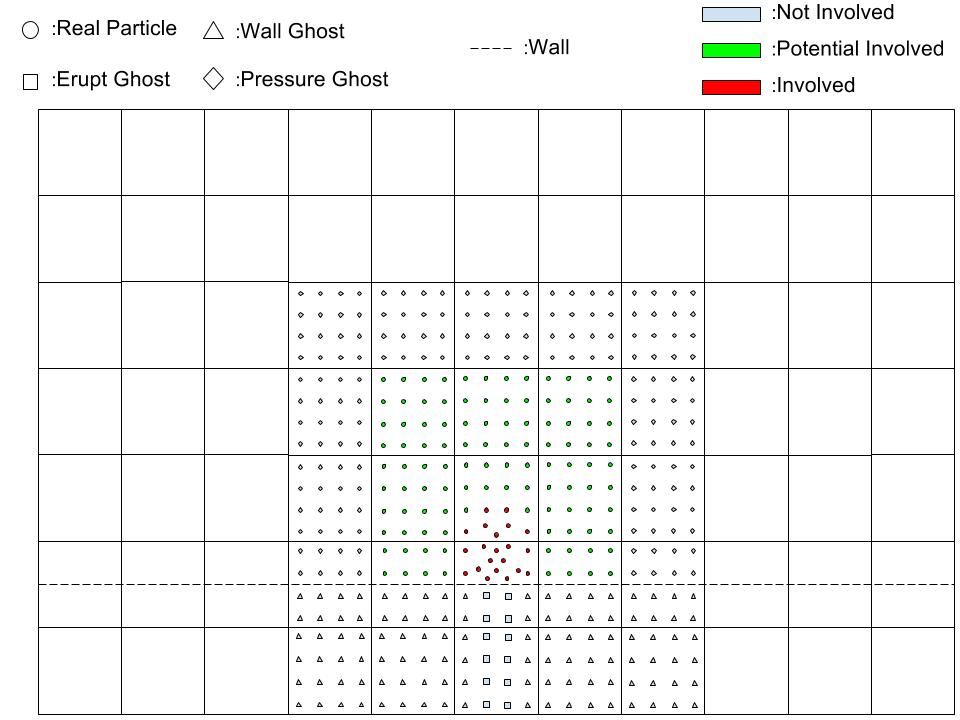
\includegraphics[width=0.5\textwidth]{Involved_initial}
\end{figure}

\begin{figure}[h]
\caption{Adjusting of domain}
\centering
\label{fig:Involved_domain_adjusting}
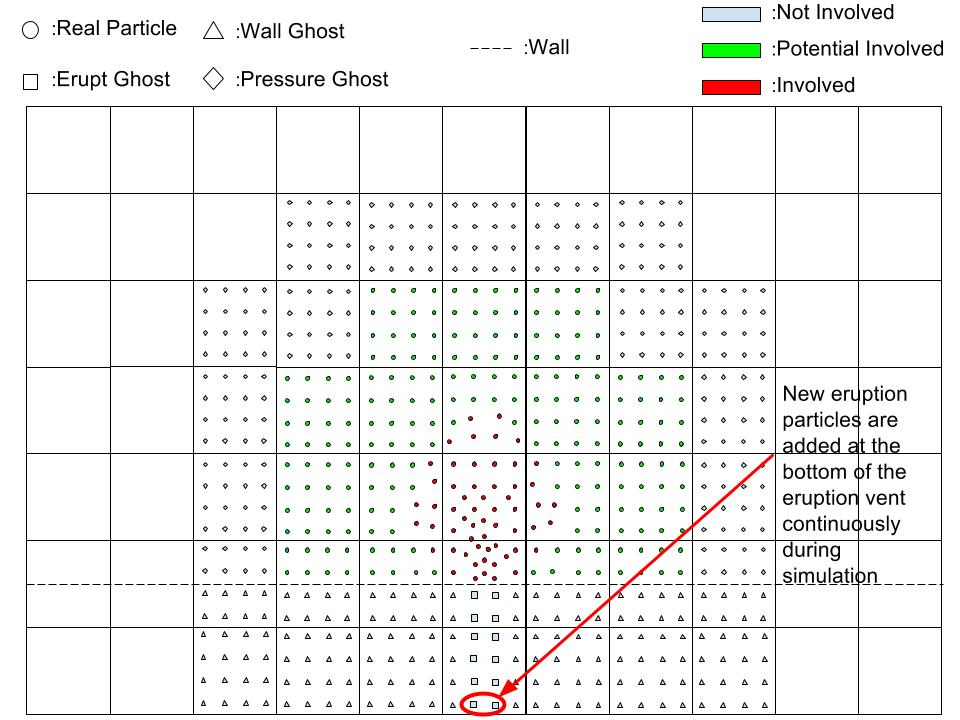
\includegraphics[width=0.5\textwidth]{Involved_domain_adjusting}
\end{figure}
}

A has-involved-flag is added in bucket class. Buckets are also categorized into 3 types based on particles they contain: has involved (has-involved-flag=3), has potential involved(has-involved-flag=1) and has no involved (has-involved-flag=0). Bucket that has any involved particle will be set to be has involved (has-involved-flag=3). And all of its neighbor buckets will be set to be has potential involved. 
All particles in has involved buckets or has potential involved buckets will be set to be potential involved except for involved particles. There are two situations that will make a has potential involved bucket to be a has involved bucket. First, when a involved particle enters a has potential involved bucket. Second, when mass fraction of a particle (It should be a potental involved particle) exceeds the threshold, this particle will turn to a involved particles and if this is the first involved particle in the bucket, the bucket will turn from a has potential involved bucket to a has involved bucekt.\\
The most outside buckets layer of has-potential-involved buckets will be scaned every time after updating. If any a of these buckets becomes has involved, the domain will be enlarged by turnning the pressure ghost particles to real particles and turning involved-flag from 0 to 1. Also, the buckets that originally contain pressure ghost particles will become has potential involved. New pressure ghost particles and wall ghost particles will be added around the adjusted domain.
This process of domain adjusting is show in figure \ref{fig:Involved_initial} and \ref{fig:Involved_domain_adjusting}.
The work flow with domain adjusting is in figure \ref{fig:Work_flow_adjust} 

For the test problem in this paper, the volcanic plume will finally reach to a domain of $[-10km \,\,\, 10km] \times [-10km\,\,\,10km] \times [0km\,\,\,20km]$ after around 300 seconds of eruption. When numerical simulation goes up to 90 seconds, the plume is still within a domain of $[-3km\,\,\,3km] \times [-3km\,\,\,3km] \times [0km\,\,\,6km]$. Adjusting of domain can avoid computing large number of uninfluenced air particles. Numercial test shows that simulation time is reduce to $\frac{1}{4}$ of original simulation time when we adopt the domain adjusting strategy in our code.
\section{Numerical test}
As we are targeting at developing data management and paralell strategies for more complicated implementation of SPH which demmands quick and flexible data access, delete and add. The test problem should have such demand. Volcanic eruption which is essentially a mutilple phases, turbulent, ejection mixing flow accompanied with microphysics processes requires more flexibile data management. We adopt a two phase volcanic plume model\citep{suzuki2005numerical} as our test problem. One phase is air while another phase is ejected material.
\subsection{Governing equations\citep{suzuki2005numerical} and boundary conditions}
Based on Navier-Stokes equations, the following assumptions are made:
\begin{itemize}
\item Molecular Viscosity is neglected since eddy viscosity due to turbulence is dominant. As heat conduction is much smaller than turbulent heat exchange \citep{oberhuber1998volcanic}, We only consider turbulent heat exchange.
\item Erupted material consist of solid with different size and mixture of gas (various constituent) is assumed to be well mixed and behave like a single phase fluid (phase 2). Air (also a mixture of different gas) is assumed to be another phase (phase 1).
\item We assume immediate thermodynamic equilibrium so that no separate energy equation is needed for each phase. As a result, there is only one energy equation for both phases and heat transfer effect between different phases will be ignored.
\item We assume immediate dynamic equilibrium so that no separate momentum equation is needed for each phase. As a result, there is only one vector moment equation for both phases. Drag force term will not show up in the momentum equation as two phases always move with the same velocity.
\item Because of above assumptions, all other micro-physics process (like phase change of $H_2O$, aggregation, decomposition, absorption of gas on the surface of solid, solution of gas into the liquid) and chemical process will not be considered in this model.
\end{itemize}
Finally the governing equations for this model in Eulerian form are:
\begin{align}
\dfrac{\partial \rho}{\partial t} + \nabla \cdot (\rho \textbf{v}) = 0 \label{eq:gov-cs-rho}\\
\dfrac{\partial \rho \xi}{\partial t} + \nabla \cdot (\rho \xi \textbf{v}) = 0 \label{eq:gov-cs-ks} \\
\dfrac{\partial \rho \textbf{v}}{\partial t} + \nabla \cdot (\rho \textbf{v} \textbf{v} + p\textbf{I}) = \rho \textbf{g} \label{eq:gov-cs-v} \\
\dfrac{\partial \rho E}{\partial t} + \nabla \cdot [(\rho E + p )\textbf{v}] = \rho \textbf{g} \cdot\textbf{v} \label{eq:gov-cs-e}
\end{align}
$\xi$ is the mass fraction of ejected material.
$E = e + K $ is total energy which is summation of kinetic energy $K$ and internal energy $e$.
An additional equation is required to close the system. In this model, the equation for closing the system is an EOS:
\begin{align}
p = (\gamma_m - 1)\rho e \label{eq:EOS}\\
\end{align}
Where 
\begin{align}
\gamma_m = R_m/C_{vm} + 1 \label{eq:gov-gm}\\
Rm = n_gR_g + n_aR_a  \label{eq:gov-Rm}\\
C_{vm} = n_s C_{vs} + n_g C_{vg} + n_a C_{va} \label{eq:gov-Cvm}\\
n_a = 1 - \xi \label{eq:gov-na}\\
n_g = \xi n_{g0} \label{eq:gov-ng}\\
n_s = \xi - n_g \label{eq:gov-ns}
\end{align}
Where, $C_v$ is specific heat with constant volume, $n$ is mass fraction, $R$ is gas constant. The subscription $m$ represents mixture of ejected material and air, $s$ is solid portion in ejected material, $g$ is gas portion in the ejected material and $a$ is air.\\

In current model the initial domain is a 3D box. The boundaries are categorized into eruption vent (a circle area at the center of the bottom), wall boundary (box bottom), pressure boundary (Other faces of the box).
At the vent, $T$, $\textbf{v}=\{0,0,150\}^T$, $p=1.01\times10^5 Pa$, $n_{g0}=0.05$ and mass discharge rate $\dot M$ is given. The radius of vent is determined from $\rho$, $\dot M$ and $\textbf{v}$.
Velocity is zero for non-slip wall boundary. We assume the boundary to be adiabatic and the heat flux is zero on the bounday. The pressure of the surrounding atmosphere is specified on pressure boundaries. Except for the pressure, boundary condtions for density, velocity, and energy will depend on the solution. We adpot ghost particles to impose these different type of boundary conditions (see figure \ref{fig:Involved_initial} and figure \ref{fig:Involved_domain_adjusting}). 
\subsection{Discretized governing equations with SPH}
There are several review papers \citep{monaghan1992smoothed, monaghan2005smoothed, price2012smoothed, rosswog2009astrophysical, monaghan2012smoothed} which provide a pretty comprehensive view over SPH. We will not cover these basic theory of SPH in this paper.
The discretized governing equations with SPH are:
\begin{align}
<\rho_a^a>=\sum m_b w_{ab} (h_a) \label{eq:gov-sph-d1}\\
<\rho_i^{sg}>=\sum_j m_j w_{ij} (h_i) \label{eq:gov-sph-d2}
\end{align}
\begin{equation}
<\dfrac{d \textbf{v}_{\alpha}}{d t}>= 
-\sum_b [m_b (\dfrac{p_b}{\rho_b^2} + \dfrac{p_{\alpha}}{\rho_{\alpha}^2} + \Pi_{\alpha b}) \bigtriangledown_{\alpha}w_{\alpha b}(h_{\alpha})]
-\sum_j [m_j (\dfrac{p_j}{\rho_j^2} + \dfrac{p_{\alpha}}{\rho_{\alpha}^2} + \Pi_{\alpha j}) \bigtriangledown_{\alpha}w_{\alpha j}(h_{\alpha})]
+\textbf{g} \label{eq:gov-sph-v}
\end{equation}

\begin{equation}
<\dfrac{d e_{\alpha}}{d t}>=
 0.5\sum_b [m_b \textbf{v}_{\alpha b}(\dfrac{p_b}{\rho_b^2} + \dfrac{p_{\alpha}}{\rho_{\alpha}^2} + \Pi_{\alpha b}) \bigtriangledown_{\alpha}w_{\alpha b}(h_{\alpha})]
 +0.5\sum_j [m_j \textbf{v}_{\alpha b}(\dfrac{p_j}{\rho_j^2} + \dfrac{p_{\alpha}}{\rho_{\alpha}^2} + \Pi_{\alpha j}) \bigtriangledown_{\alpha}w_{\alpha j}(h_{\alpha})] \label{eq:gov-sph-e}
\end{equation}
Where
$\rho_a^a$ is density of phase 1 (air).
$\rho_i^{sg}$ is density of phase 2 (erupted material).
$\rho=\rho^a + \rho^{sg}$ is density of mixture of phase 1 and phase 2.
\begin{align}
\textbf{v}_{\alpha b}=\textbf{v}_{\alpha}-\textbf{v}_b \\
\textbf{v}_{\alpha j}=\textbf{v}_{\alpha}-\textbf{v}_j
\end{align}
$w_{ab} (h_a)= w(\textbf{r}_a-\textbf{r}_b,h_a)$ is smoothing kernel.
%$\bigtriangledown_{\alpha}w_{\alpha j}(h_{\alpha})$-->need double check
$\Pi$ is artificial viscosity term \citep{monaghan1992smoothed}.
Index $a$, $b$ is for phase 1.
Index $i$, $j$ is for phase 2.
Index $\alpha$, $\beta$ can be index of either phase 1 or phase 2.
The position of each particle is updated according to the following equation.
\begin{align}
\dfrac{d \textbf{r}_a}{dt} = \textbf{v} \label{eq:gov-update-pos}
\end{align}
Free surface flow are in nature turbulent. We adopt $SPH-\varepsilon$ method developed by Monaghan\cite{monaghan2011turbulence} to capture turbulence in the plume. This will result to a filtered velocity for position updating and additional turbulent terms in momentum and energy eqution.
\subsection{Solver performance}
Experiments have been carried out on the computational cluster of Center for Computational Research (CCR) at Buffalo. The initial domain is $[-4800m,4800m]\times [-4800m,4800m] \times [0, 4000]$, with smoothing length of 200m. The computation was run for 20s physical time. The running time and speed up are shows in figure \ref{fig:performance_128_time} and \ref{fig:performance_128_speed_up}. The results shows very good strong scalability when number of processes is smaller than 64. A overhead of scalability also shows up in the figure. The over head of speed up is due to 2D domain decomposition. For this test case, the total number of footprint buckets in x-y plane is 64. Recall that domain decomposition 2D and is based on SFC of footprint buckets. When we request 128 processes but there is only 64 buckets initially, another 128 processes will be totally idle at the beginning. As simulation goes, the domain is expanded and more and more idle processes will start getting tasks. That's why we still get some speed up. This can be easily demonstrated by another experiment with more buckets on x-y plane. In our second experiment, we still use the same domain, but we take smoothing length as 100m. As a reseult, there will be 256 footprint bucekts on the x-y plane initially. The results are consistent with our expectation: we got linear speed up up to 256 processes. Adgain, the an overhead shows up when number of processes is larger than 256. This motivate us to adopt three dimensional domain decomposition in our future research.
\begin{figure}[h]
\caption{Running time Vs number of processes}
\centering
\label{fig:performance_128_time}
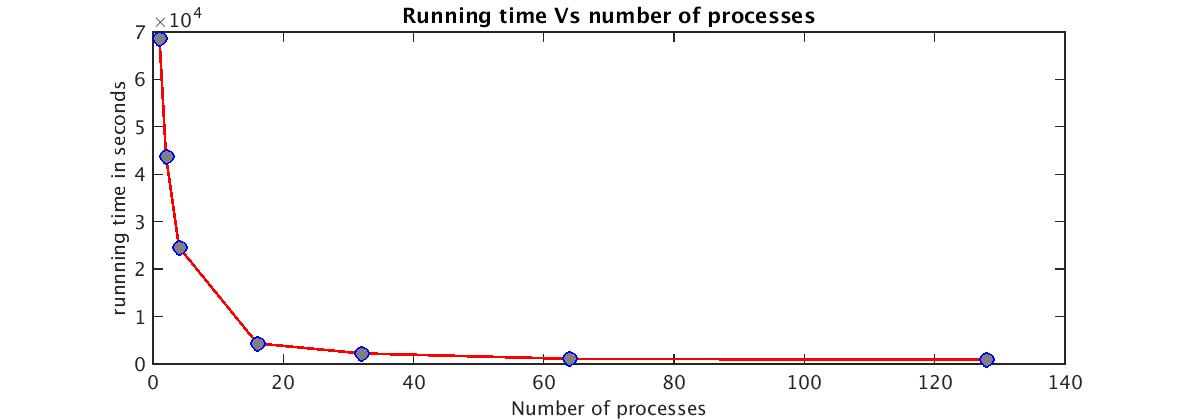
\includegraphics[width=0.7\textwidth]{128_time}
\end{figure}
\begin{figure}[h]
\caption{Speed up: Strong scalability}
\centering
\label{fig:performance_128_speed_up}
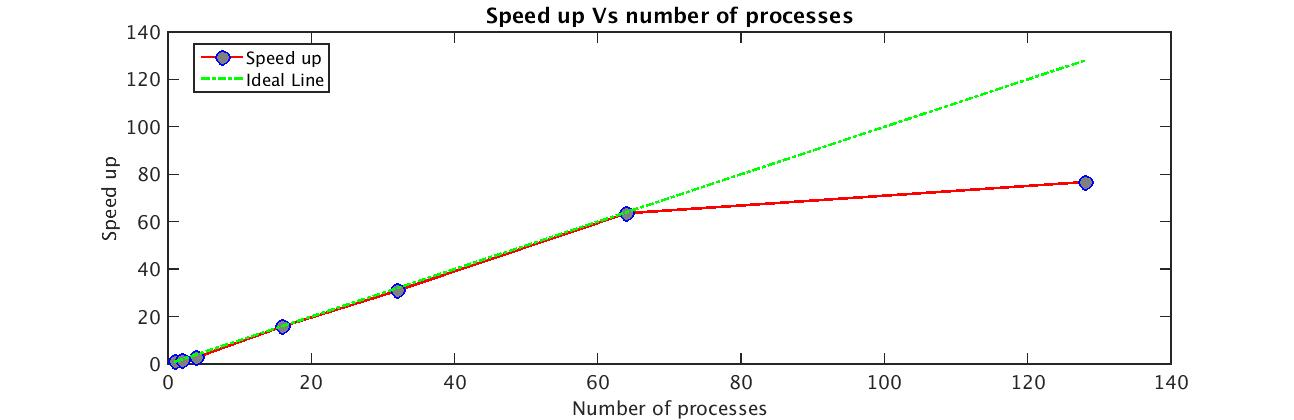
\includegraphics[width=0.7\textwidth]{128_speed_up}
\end{figure}

\section{Conclusion}
We developed data management strategies for parallel implementation of SPH method using MPI standard to simulate complicated problems, such as JUPE, which requires flexible and fast data retrievalling, adding and deleting. Neighbors searching and domain decomposition is based on background grid which overlaps the domain and keep stationary during simulation. SFC based index scheme, which provides a global numberring methodology that is purely coordinates dependent, is adopted to give each bucket an unique identifier. A time dependent key which is also based on SFC is used as identifier for particles. 
Hashtables with external link list are adopted for accessing  particles and buckets data. Based on weighted particle work load, a dynamic load balance strategy is developed by checking load balance and redecomposing the domain at an optimize interval. The code was further improved to 4 times faster by adjusting computational domain according to progress of simulation. 
Our code shows a linear speed up and an overhead cast by number of footprint buckets in x-y plane. This motivate us to adopt three dimensional domain decomposition in our future research.

\bibliographystyle{plainnat}
\bibliography{Reference}

\end{document}